\documentclass[10pt,a4paper]{article}
\usepackage[utf8]{inputenc}
\usepackage[spanish]{babel}
\usepackage{amsmath}
\usepackage{amsfonts}
\usepackage{amssymb}
\usepackage{graphicx}
\usepackage{multicol}
\usepackage{titling}
\usepackage{titlesec}
\usepackage{array}
\usepackage{bm}
\usepackage{afterpage}
\usepackage{booktabs} %LIBRERIA PARA EXCE
\usepackage{multirow}
\usepackage{float}
\usepackage{pdfpages}
\usepackage{graphicx}
\usepackage{epstopdf}
\usepackage{longtable}
\usepackage{xcolor}
\usepackage[spanish]{babel}
\usepackage[utf8]{inputenc}
\usepackage[spanish]{babel}
\usepackage[utf8]{inputenc}
\usepackage{tikz}
\usepackage{verbatim}
\usepackage{smartdiagram}

\usepackage{multirow}


\usetikzlibrary{shapes,arrows}
\usepackage{color}
\usepackage{epigraph}
\setlength\epigraphwidth{1.5\textwidth}
\usepackage{subfigure}
\usepackage{anyfontsize}
\usepackage[left=2cm,right=2cm,top=2cm,bottom=2cm]{geometry}

\usepackage[colorlinks=true,
            linkcolor=blue,
            citecolor=blue,
            urlcolor=blue]{hyperref}

\begin{document}
\author{Cauja María José, Chandi Armando, Nazate Marisol, Valencia Fernando} % CAMBIAR A AUTORES
\title{\textbf{CALIDAD DEL AIRE}}
\date{10 de enero de 2020}
\maketitle  

\section{Introdución}

Actualmente la polución ambiental es uno de los principales problemas a nivel mundial. Debido a las altas concentraciones de contaminación atmosférica se presentan efectos negativos para la ciudadanía, a causa de los contaminantes nocivos se registra una mayor tasa de enfermedades y problemas respiratorios. En consecuencia se presentan efectos económicos considerables, ya que acorta la vida, aumenta los costes médicos y reduce la productividad. Por lo tanto es necesario usar un medidor de calidad del aire, pues de esa manera se puede tomar las precauciones necesarias para evitar ese tipo de problemas o al menos reducir en gran parte los efectos negativos.
La contaminación ambiental ha ido en crecimiento, por lo cual causa grandes pérdidas  a nivel mundial, como a nivel social, económico y de salud, por lo que se ha visto la necesidad de realizar la implementación de un sistema que pueda medir la calidad del aire. El principal objetivo es realizar un análisis de la calidad del aire en varios puntos de muestreo más considerables y representativos para la obtención de datos reales, útiles y que presenten margen de error en cantidades mínimas. Uno de los principales métodos de solución que contribuyen a la calidad del aire y efectos sobre la salud son las redes inalámbricas de sensores.\\
A continuación se realizará un breve análisis de algunos de los sistemas que se pueden utilizar. Actualmente se utilizan varios sensores para supervisión de agentes contaminantes en el aire con el fin de determinar el grado de pureza de oxígeno y como este influye en una población específica, un ejemplo son los sensores de quimioluminiscencia los cuales ejecutan un principio de medición que se basa en la reacción radioactiva del ozono con óxido de nitrógeno (NO) permitiendo medir su cantidad, otro agente externo es el NOx (x puede ser cualquier valor) el cual se puede medir mediante la separación de NO por la luz UV (ultravioleta). Por otro lado se tiene el impacto de la emisión de NOx en el clima y el monitoreo utilizando tecnología de sensores inteligentes Este es un sistema que se plantea para desarrollar un clasificador inteligente de monitorización y control de la calidad de combustión de temperatura y NOx. El principal objetivo es la detección, el reconocimiento y comprensión de las condiciones de combustión mediante la utilización de sensores inteligentes, los cuales son operados y controlados por un sistema basado en análisis de datos con un límite umbral. Otro de los sistemas propuesto es el llamado Pulluino, el cual corresponde a una gestión eficiente basada en la nube de dispositivos IoT para monitoreo de calidad del aire Es un sistema que sirve para el control de la contaminación del aire, mediante una eficiente nube basada en gestión de dispositivos IO para el monitoreo del aire.\\
Estos dispositivos inteligentes son capaces de detectar, almacenar y analizar los flujos de datos en una red de información y comunicación. Dentro de los diversos sistemas se tiene también el desarrollo de plataforma de detección para mediciones y análisis de calidad del aire para obtener datos acerca de la calidad del aire a partir de un ensamblaje de bajo costo en Arduino el cual muestra los datos de una forma simple en una pantalla LCD así mismo permite visualizar índices de contaminación en función a la combinación de luces LED, este sistema capturó datos de SPM (partículas suspendidas), NRMF (el respirable de las partículas suspendidas), SO2, etc; los cuales pueden ser utilizados para un posterior estimaciones de contaminación a la que están expuestos los seres vivos. Finalmente se tiene el sistema de monitoreo de contaminación de aire urbano con modelos de predicción debido a que este sistema utiliza sensores gaseosos y meteorológicos que realizan el monitoreo del nivel de contaminación en el aire de una zona urbana determinada, los datos adquiridos se envían a una base de datos la cual procesaría y mostraría únicamente los datos que puedan servir como información útil para una posterior predicción del nivel de contaminación. Todos estos sistemas son indicados para determinar la detección de posibles malas condiciones ambientales, pues es de gran relevancia debido a que es capaz de contribuir a varios campos de aplicación y sectores del mercado especialmente para mejorar las condiciones medioambientales y por ende la calidad de vida.

\section{Diseño del sistema}
\subsection{Placa del sistema}

Para el desarrollo del siguiente proyecto se usará una placa de desarrollo MCU, en conjunto con Arduino Uno, los cuales nos permitirá realizar las conexiones de los diferentes sensores.
Se ensamblará los diferentes sensores en una baquelita, diseñando así las pistas de las conexiones que corresponden para cada uno de los dispositivos.

\subsection{Conexiones}

Se debe tener en cuenta un diseño de conexiones de todos los dispositivos para el funcionamiento del sistema, se crea en el software libre Fritzing siendo un programa que nos permite hacer esquemas eléctricos, y diseñar nuestro PCB final.

\begin{figure}[H]
\centering
 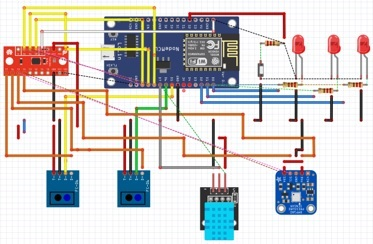
\includegraphics[scale=0.80]{fritzingcorregido.JPG} 
\caption{Diseño en Fritzing} 
\end{figure}

\begin{figure}[H]
\centering
 \includegraphics[scale=0.80]{diagramaesquematico.JPG} 
\caption{Diagrama Esquemático} 
\end{figure}

Las conexiones que se realizan constan de: tres leds con sus respectivas resistencias los cuales nos permitirá revelar los diferentes parámetros, y los diferentes enlaces de los sensores NodeMCU, DHT11, MQ-135, y Sensor Rayo UV GYM L8511

\subsection{Diagrama de conexión }

Para la realización del diagrama de pistas en la PCB, se lo ejecuto en el software PCB Wizard, siendo aquel que permite crear esquemas de circuitos electrónicos y a partir de estos, obtener de una manera sencilla el diseño del circuito impreso a una o dos caras

\begin{figure}[H]
\centering
 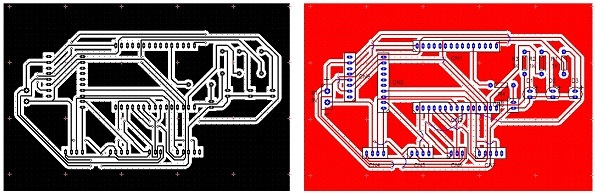
\includegraphics[scale=0.68]{placasensores.JPG} 
\caption{Pista esquemática PCB} 
\end{figure}

El proceso de fabricación de una placa PCB, se lo realizo con una impresión laser del circuito en papel couche, luego se lo recorta el circuito del tamaño necesario que necesita la lámina circuital, para consiguiente planchar el recorte sobre la baquelita de cobre, siendo que la tinta a laser y el papel couche, se quede impregnada en la placa por el calor; finalmente a la baquelita se lo pone en acido por unos minutos, y por siguiente el cobre sobrante se eliminando, quedando así las pistas conductoras de cobre. 


A continuación de este proceso se realizan las perforaciones con taladro de broca delgada, teniendo cuidado que las pistas puedan ser afectadas.\\


\section{Desarrollo}

\subsection{Diagrama de Bloques}


\begin{center}
\smartdiagramset{
uniform color list=gray!60!black for 1 items,
back arrow disabled=true,
}
\smartdiagram[flow diagram:horizontal]{Node MCU/8266,Multiplexor /74HC4051, DTH11, MQ135, Sensor /RayosUV, Resistencias /Leds Indicadores}
\end{center}


\subsection{Selección de los sensores}

Para poder escoger entre estos sensores se procedió a comparar con varios tipos; existen diferentes opciones tanto genéricas como profesionales para efectos del proyecto serán necesarios sensores que puedan obtener datos de aire, humedad y temperatura.\\\\

\textbf{Placa NodeMCU}\\

Es de código abierto basado en el chip ESP8266 (ESP-12E), que utiliza el lenguaje de programación Lua para crear un ambiente de desarrollo para aplicaciones que requiera conectividad Wifi de manera rápida.
El ESP8266 ofrece una solución completa y autónoma de redes Wi-Fi, lo que le permite alojar la aplicación o servir como puente entre Internet y un microcontrolador, tiene potentes capacidades a bordo de procesamiento y almacenamiento que le permiten integrarse con sensores y dispositivos específicos de aplicación.\\\\

\textbf{Sensor DHT-11}\\

El DHT11 es un sensor de humedad relativa y temperatura de bajo costo y de media precisión. Integra un sensor capacitivo de humedad y un termistor para medir el aire circundante, y muestra los datos mediante una señal digital en el pin de datos . \\\\\\\\

\textbf{Sensor MQ-7}\\

Este sensor es de alta sensibilidad al monóxido de carbono (CO), pero también es sensible al H2.  Puede detectar concentraciones en el rango de 20 a 2000ppm.
El módulo posee una salida analógica que proviene del divisor de voltaje que forma el sensor y una resistencia de carga. También tiene una salida digital que se calibra con un potenciómetro, esta salida tiene un led indicador.

\begin{table}[t]
\begin{center}
\begin{tabular}{| c | c | c | c |}  
\hline
 
\textbf {Tipo Sensor} & \textbf {Parámetro} &  \textbf {Rango de Medida} & \textbf  {Valores Obtenidos} \\  \hline
Sensor MQ-7 & Monóxido de Carbono (CO) & 20 a 2000ppm & 657 ppm \\ \hline
\end{tabular}
\caption{ MQ-7.}
\end{center}
\end{table}
Para hacer conversión de unidades de concentración de partes por millón (ppm), a microgramos por metro cúbico (ug/m3) se aplicará la siguiente ecuación\\
\begin{equation}
\frac{ug}{m^{3}}= \frac{ppm * PM}{24.5}*10^{3}
\end{equation} \\

\begin{table}[htb]
\begin{center}
\begin{tabular}{| p{2.2cm}| p{4.2cm} | p{6.2cm}| }
\hline
\multicolumn{3}{|c|}{Partículas menores a 10 micrómetros (PM10)} \\
\hline
Índice & Concentración & Ecuaciones \\
\hline \hline
Intervalo  & Intervalo de Concentración ug/m3 & Ecuaciones  \\ \hline
0-50 & 0 – 40 & I(PM10) = 1,25x C(PM10) \\ \hline
51- 100 & 41 – 75 & I(PM10) = 1,44x(C(PM10)-41) +51 \\ \hline
101- 150 & 76 – 214  & I(PM10) = 0,355x(C(PM10)-76) +101 \\ \hline
151-200 & 215 – 354 & I(PM10) = 0,353x(C(PM10)-215) +151 \\ \hline
mayor a 200	& mayor a 354 & I(PM10) = 0,567x C(PM10) \\ \hline
\end{tabular}
\caption{PM10.}
\end{center}
\end{table}

\textbf{Sensor MQ-135}\\

Se utilizan en equipos de control de calidad del aire para edificios y oficinas, son adecuados para la detección de NH3, NOx, alcohol, benceno, humo, CO2, etc
Este sensor no proporciona valores absolutos, sino que simplemente proporciona una salida analógica que debe ser monitoreado y se comparada con los valores de umbral.


\begin{table}[htb]
\begin{center}
\begin{tabular}{| c | c | c | c |}  
\hline 
\textbf {Tipo Sensor} & \textbf {Parámetro} &  \textbf {Rango de Medida} & \textbf  {Valores Obtenidos} \\  \hline
Sensor MQ-135 & Amoniaco (NH3) Sulfuro Benceno (C6H6) Humo  & De 10 ppm a 1000 ppm & 300 ppm \\ \hline
\end{tabular}
\caption{ MQ-135.}
\end{center}
\end{table}

Se presentan las fórmulas para calcular el Índice, a partir de concentración de los contaminantes, ya sea en partes por millón (ppm) o en microgramos por metro cúbico.\\

\begin{longtable}{| p{2.2cm}| p{4.2cm} | p{6.2cm}| }
\hline
\multicolumn{3}{|c|}{Partículas menores a 2.5 micrómetros (PM2.5)} \\
\hline
Índice & Concentración & Ecuaciones \\
\hline \hline
Intervalo & Intervalo de Concentración ug/m3 & Ecuaciones \\ \hline
0-50 & 0-12 & I(PM2.5) = 4.17x C(PM2.5)) \\ \hline
51- 100 & 12.1 -45 & I(PM2.5) = 1.49x(C(PM2.5)-12.1) +51 \\ \hline
101- 150 & 45.1-97.4 & I(PM2.5) = 0.94x(C(PM2.5)-45.1) +101 \\ \hline
151-200 & 97.5-150.4 & I(PM2.5) = 0.93x(C(PM2.5)-97.5) +151 \\ \hline
mayor a 200 & mayor a 150.4 & I(PM2.5) = 1.335x C(PM2.5) \\ \hline
\caption{ PM 2.5.}
\end{longtable}


\textbf {Sensor Rayos UV GYML8511}

Este sensor UV, se utiliza para detectar el índice de intensidad ultravioleta (UV). Tiene una amplia gama espectral de 200nm hasta 370nm*. La señal eléctrica de salida del módulo es de tipo analógica, que varía respecto a la intensidad de los rayos \\\\\\\\\\

\subsection{Tabla de datos}

\begin{longtable}{| c | c | c | c |}  
\hline
\textbf {Tipo Sensor} & \textbf {Parámetro} &  \textbf {Rango de Medida} & \textbf  {Valores Obtenidos} \\  \hline
 Rayos UV GYM L8511 & UV & Índice mayor a 12 (extremadamente alto) & Entre un índice de 3 a 4  \\ \hline
\caption{Valores de sensores en rangos de medida y valores obtenidos.}
\end{longtable}


Modo nucleación: Tamaño menor de 20 nm \\

PM10: Partículas con diámetro aerodinámico menor de 10 um \\

Para hacer conversión de unidades de concentración de partes por millón (ppm), a microgramos por metro cúbico, se aplicará la siguiente ecuación
	
\begin{equation}
\frac{ug}{m^{3}}= \frac{ppm * PM}{24.5}*10^{3}
\end{equation} 

\section{Simulación y gráficos de adquisición de datos }
\subsection{Filtro de mediana}

El filtro de mediana define una ventana de N elementos, que recoge las últimas N mediciones. El valor del filtro es la mediana de los valores contenidos en la ventana.
Aumentar el tamaño de la ventana aumenta el suavizado de la señal pero añade un retraso a la señal ya que es necesario "esperar" al muestreo de más puntos, se prefieren tamaños de ventana impares para evitar tener que promediar entre dos muestras, lo cual eliminaría parte de la capacidad de filtrado de la mediana. Siendo su formula:

\begin{equation}
z_{j}=median (x_{j-n}..x_{j-2},x_{j-1},x_{j},x_{j+1},x_{j+2}...x_{j+n})
\end{equation}

Para encontrar la mediana, las muestras de la ventana N-muestras se ordenan y la mediana se determina como:

\begin{equation}
\begin{Bmatrix}
S_{(n+1)/2} , & if  & N & mod 2==1 & \\
S_{N/2-1}+S_{N/2+1}, & if  &  N &  mod 2==1 & 
\end{Bmatrix}
\end{equation}

La fórmula describe la selección de la mediana de la lista ordenada S. si N es impar, la mediana es la muestra 
\begin{equation}
 S_{(n+1)/2} 
\end{equation}
 entonces la mediana es el promedio de dos elementos 
\begin{equation}
S_{N/2-1}  
 \end{equation} 
\begin{equation}
S_{N/2+1}
 \end{equation} 

\subsection{Filtro Mediana}
En los resultados presentes como se puede apreciar en la primera figura se mostrará el filtro del sensor MQ7, se ve que se ha quitado la mayoría de los picos de la señal, lo que se corresponde para la eliminación de espurios y ruido, también se visualiza que existe un pequeño retardo con respecto a la señal original de igual forma en el sensor MQ135 y UV GYML8511.
Para el sensor MQ135 siendo este el que detecta los gases CO y CO2, el suavizado de la señal es mas visible ya que los datos extraídos tienen más variación de mínimos y máximos con relación al sensor anterior, mientras que para el sensor UV GYML8511, al tener una escala de normalidad entre 0-15 el filtrado en este caso al contener datos de magnitudes muy pequeñas pues la señal será casi nula, y se podrá visualizar en los picos más altos. El suavizado es producir cambios lentos en el valor para que sea más fácil ver las tendencias en nuestros datos.\\

Señal de datos de entrada 
Sensor: MQ7  Datos de muestra: 449 datos de variación de CO
Interpretación:  Línea azul – Datos, Línea roja- señal suavizada 

\begin{figure}[H]
\centering
\includegraphics[scale=0.65]{mediana1.JPG}
 \caption{Filtro mediano para sensor MQ7} 
\end{figure} 

Señal de datos de entrada 
Sensor: MQ135  Datos de muestra: 449 datos de variación de CO2
Interpretación:  Línea azul – Datos, Línea roja- señal suavizada 

\begin{figure}[H]
\centering
\includegraphics[scale=0.65]{mediana2.JPG}
 \caption{Filtro mediano para sensor MQ135} 
\end{figure} 

Señal de datos de entrada 
Sensor: UV GYML8511 		
Datos de muestra: 449 datos de variación de concentración de rayos UV es escala 0-15
Interpretación: Línea azul – Datos, Línea roja- señal suavizada 

\begin{figure}[H]
\centering
\includegraphics[scale=0.65]{mediana3.JPG}
 \caption{Filtro mediano para sensor UV} 
\end{figure} 


\section{Diseño de Placa y Pruebas de Funcionamiento}
\subsection{Diseño de Placa}

\begin{figure}[H]
\centering
\includegraphics[scale=0.65]{pistaplaca.JPG}
 \caption{Pista de Placa} 
\end{figure} 

\begin{figure}[H]
\centering
\includegraphics[scale=0.85]{implementacionplaca.JPG}
 \caption{Implementación de los componentes} 
\end{figure} 


\section{Análisis de datos, gráficas y desarrollo en R}

Para poder utilizar este método de evaluación de un modelo de clasificación necesitamos separa nuestra data de entrenamiento en dos datasets.\\
Entrenamiento (80 por ciento)\\
Pruebas (20 por ciento)\\
Lo que haremos es entrenar el modelo utilizando las observaciones que están en el dataset train y luego evaluaremos el modelo utilizando las observaciones del dataset test.\\
Esto nos ayudar a medir como se comporta nuestro modelo cuando se lo aplicamos a data nueva. La matriz tiene la siguiente estructura, a continuación, se muestra el resultado de la separación de datasets de un total de 782 muestras definidas en 3 etiquetas.

\begin{figure}[H]
\centering
\includegraphics[scale=0.85]{data.JPG}
 \caption{Base de entrenamiento y test} 
\end{figure} 


\subsection{Normalizacion de Datos }

\begin{figure}[H]
\centering
\includegraphics[scale=0.85]{library.JPG}
 \caption{Datos normalizados} 
\end{figure} 

\subsection{Algoritmo KNN}
Con k=15, la eficiencia del algoritmo es del 100 por ciento es comparación de utilizar los valores no normalizados donde la eficiencia era de 98 por ciento.

\begin{figure}[H]
\centering
\includegraphics[scale=0.85]{confusion.JPG}
 \caption{Matriz de confusión KNN} 
\end{figure}

\subsection{Clasificador Bayesiano}

La eficiencia mejoro notablemente, mostrando una diagonal exacta en reconocimiento de valores de la etiqueta 1 de la matriz de prueba con relación a la etiqueta 1 de la matriz de entrenamiento. 

\begin{figure}[H]
\centering
\includegraphics[scale=0.85]{bayesiano.JPG}
 \caption{Clasificador Bayesiano} 
\end{figure}


\subsection{CNN}

Con el fin de mejorar el algoritmo se aplica una reducción de la base de datos para evaluar únicamente datos válidos, la matriz de entrenamiento se redujo de 626 datos a 611 es decir que del valor anterior de datos se desprecia el 2.3962 por ciento. 

\begin{figure}[H]
\centering
\includegraphics[scale=0.85]{instancia.JPG}
\includegraphics[scale=0.85]{instancia1.JPG} 
\caption{Eliminación de Instancias} 
\end{figure}




\section{Interfaz}

La interfaz fue diseñada con el objetivo de tener una mejor interacción entre el usuario y el prototipo, con el cual se ha creado de una manera dinámica en el que se podrá observar tanto los componentes contaminantes como el estado del ambiente que se analiza.\\

La plataforma esta constituida por dos botones: desconectar, será aquel que habilita el sistema para empezar a realizar el análisis; mientras que el botón guardar nos dará la opción de poder crear una tabla de los datos de los sensores para el estudio profundo con respecto a los contaminantes del aire. También se implementa un medidor de la calidad del aire siendo 0.0 puro y 5.0 contaminante.

\begin{figure}[H]
\centering
\includegraphics[scale=0.85]{interfaz1.JPG}
\caption{Interfaz} 
\end{figure}

\section{Conclusiones y Recomendaciones}
\subsection{Conclusiones}

El sensor de dióxido de carbono MQ135 necesita de 5 a 10 minutos para calibrarse al ambiente y estabilizar sus mediciones de dióxido de carbono, terminada la calibración estará tomando los valores de la concentración de CO2 en el ambiente cada 10 segundos y el sensor MQ7 es que la sensibilidad del sensor puede ser ajustada mediante un potenciómetro, dependiendo las necesidades del usuario.\\

Para trabajar con estas señales primero se las debe adquirir de los diferentes sensores, esto implica una etapa de acoplamiento y filtrado ya que requiere una señal lo más limpia posible, una vez realizado esto se procede a ingresarlo al microcontrolador en donde se tomara los resultados y se generara una base de datos con la cual el sistema trabajara para tomar una decisión acertada. \\

El suavizar la señal es la forma para detectar los patrones importantes en los datos extraídos de los sensores, dejando fuera el ruido que se encuentran en el sistema; teniendo como objetivo del suavizado producir cambios lentos en el valor para que sea más fácil ver las tendencias en los datos.\\

El filtro mediano es una forma sencilla de preservar los bordes de la señal original, pero aun así suavizar los niveles, el que elimina cualquier componente que sea periódico con respecto a la duración del filtro.\\

Para la reducción de la matriz de entrenamiento se utiliza el algoritmo de CNN , en la que se obtiene una comprensión de 626 datos a 611 es decir que del valor anterior de datos se desprecia el 2.3962 por ciento.\\

El software diseñador Processing que se basa en programación Java, C, fue utilizado para la realización de la interfaz con la que se ha desarrollado de una manera emprendedora, con los componentes que la aplicación nos facilita.\\


\subsection{Recomendaciones}

Se debe calibrar los sensores de manera adecuada de acuerdo a la aplicación que se desea realizar y las necesidades del usuario.\\

La toma de datos debe tener grandes variaciones para tener una mejor visualización de la señal y así mismo del filtro que se implemente. \\

Se recomienda minimizar un tipo de error de clasificación, debido a que la invariabilidad del umbral de clasificación no es conveniente debido a los casos en que hay amplias discrepancias en las consecuencias de los falsos negativos frente a los falsos positivos.\\

Para que el sistema aprenda continuamente se debe tomar valores en casos extremos, decir tomar valores en los que se puedan trabajar de una manera correcta ya que esto permitirá que el sistema sea lo más optimo posible.\\

\section{Anexos}

\begin{figure}[H]
\centering
\includegraphics[scale=0.85]{foto3.JPG}
 \caption{Grupo} 
\end{figure} 

\begin{figure}[H]
\centering
\includegraphics[scale=0.45]{foto1.JPG}
\includegraphics[scale=0.25]{placanueva.JPG}
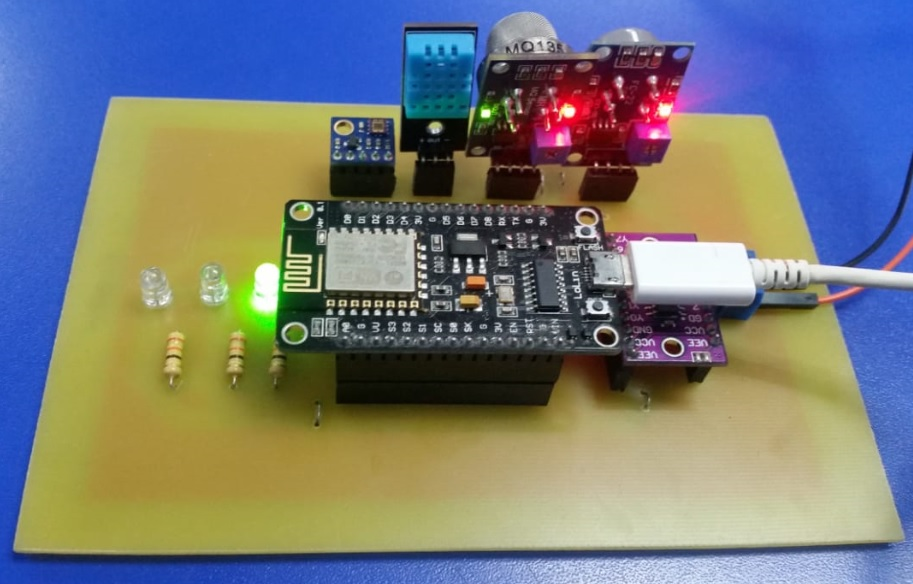
\includegraphics[scale=0.25]{placanueva1.JPG}
 \caption{Obtención de datos} 
\end{figure} 


%\section{Anexos}
%\begin{figure}[H]
%\caption{Adaptabilidad de sensores} % ingresa nombre de la figura (caption)
%\centering
%\includegraphics[scale=0.07]{Grupo.jpeg} 
%\includegraphics[scale=0.07]{Grupo2.jpeg}
%\end{figure}
%\begin{figure}[H]
%\caption{Codigo Sensores} % ingresa nombre de la figura (caption)
%\centering
%\includegraphics[scale=0.51]{Codigo1.jpg} 
%\includegraphics[scale=0.51]{Codigo2.jpg} 
%\includegraphics[scale=0.50]{Codigo3.jpg}
%\end{figure}



\end{document}
 

%\begin{thebibliography}{X}

%\bibitem{BioNo} \textsc{K. Sujatha} y \textsc{Dr. N. Pappa.},\textit{Combustion Quality Estimation in Power Station Boilers using Median Threshold Clustering Algorithms},\textit{ Science and Technology}, Vol. 2(7),2623-2631

%\bibitem {BioNo} \textsc{ D. Bandyopadhyay} y \textsc{J. Sen},\textit{Applications and Challenges in Technology and Standardization},vol. 58, no. 1, pp. 49–69, May 2011

%\bibitem{BioNo} \textsc{M. A. Hearst, S. T. Dumais, E. Osman, J. Plat} y \textsc{ B. Scholkopf},\textit{Support vector machines},\textit{ IEEE Intel},  vol. 13, no. 4,pp. 18–28, Jul./Aug. 2008.

%\bibitem{BioNo} \textsc{C. Alippi, G. Anastasi, M. D. Francesco} y \textsc{ M. Roveri},\textit{Energy
%management in wireless sensor networks with energy-hungry sensors},\textit{ IEEE Instrumentation},  vol. 12, no. 2, pp. 16–23, April 2009.

%\bibitem{BioNo} \textsc{Y. Wang} y \textsc{ K.He},\textit{The air pollution picture in China},\textit{ IEEE Spectrum},  vol. 36, no. 12, pp. 55–58, December 1999.

%\end{thebibliography}

%\section{Laboratorio}
%Laboratorio \#2\\
%\fcolorbox{black}{white}{
%\begin{minipage}[t]{16 cm}
%\textbf{Laboratorio: Manejo de sensores} 
%\end{minipage}
%}\\
%\fcolorbox{black}{white}{
%\begin{minipage}[t]{16 cm}
%\textbf{Tipo de Práctica: Diseño e Integradora}\\ 
%\textbf{Instrucciones:}\\
%*Realizar una comparación entre los diferentes sensores del mercado y elegir uno bajo los criterios de facilidad de uso, costo, librerías, entre otros. \\
%*Una vez adquiridos los sensores realizar una tabla de características del mismo.\\ 
%*Al ser sensores que tiene gran variación de los datos, buscar filtros (mínimo 3) para reducir el ruido. Plotear las diferentes respuestas para elegir al adecuado.\\ Ejemplo:\\
%\url{https://www.megunolink.com/articles/coding/3-methods-filter-noisy-arduino-measurements/}
%
%\textbf{Posicionamiento Ergonómico:}\\
%*acelerometros, sensor de distancia y presión.
%
%\textbf{Detección de estrés en estudiantes:}\\
%Elegir los sensores a usar de la plataforma mySignals de libelium. \\
%Revisar este caso de estudio
%\url{http://www.libelium.com/libelium-promotes-health-monitoring-in-the-workplace-with-mysignals/}
%
%\textbf{Detección de Calidad del Agua en Lagunas:}\\
%Revisar y adquirir los sensores:\\
%Sensor de turbidez,de calidad del agua, Ph, temperatura
%
%\textbf{Detección de Calidad del Ague en Ríos:}\\
%Revisar y adquirir los sensores:\\
%Sensor de turbidez,de calidad del agua, Ph, temperatura y distancia. \\
%
%
%Finalmente, presente el diseño en fritzing del sistema y añada su resumen realizado de las lecturas (máximo 1 hoja).
% 
%\end{minipage}
%}\\
%\fcolorbox{black}{white}{
%\begin{minipage}[t]{16 cm}
%\textbf{Presentación:} Miércoles 22 de mayo en horario de clase. 
%
%\end{minipage}
% }

%\section{Avances de Proyecto: Detección de estrés en estudiantes}
%\begin{itemize}
%\item \textbf{21/05/2019: Avance de acoplamiento}\\
%El objetivo de esta semana es tener en protoboard la mejor señal posible del sensor. Para ello, se debe realizar una selección técnica de cada sensor. Se recomienda el uso del estándar IEEE 29148 que nos indica que se debe establecer en primera instancia una situación inicial (técnica de observación) del lugar donde se implementará el sistema. Posterior a ello, se definen los requerimientos. Estos nos permiten determinar las funcionales exactas que debe tener el proyecto y sus limitaciones. Con ello, se seleccionan los sensores que serán parte del sistema. Se adjunta formato de requerimientos. Una vez adquiridos los sensores realizar una tabla de características del mismo. \\
%Al ser sensores que tiene gran variación de los datos, buscar filtros (mínimo 3) para reducir el ruido. Plotear las diferentes respuestas para elegir al adecuado.\\ Ejemplo:\\
%\url{https://www.megunolink.com/articles/coding/3-methods-filter-noisy-arduino-measurements/}

% Table generated by Excel2LaTeX from sheet 'Hoja1'
%\begin{table}[htbp]
%  \centering
%  \caption{Add caption}
%    \begin{tabular}{|l|ccc|r|r|r|r|}
%    \toprule
%    \multicolumn{4}{|c|}{Requerimientos de Funciones} & \multicolumn{3}{c|}{Prioridad} & \multicolumn{1}{c|}{\multirow{2}[4]{*}{Relacion}} \\
%\cmidrule{1-7}    \#    & \multicolumn{3}{c|}{Requerimiento de software} & \multicolumn{1}{l|}{Alta} & \multicolumn{1}{l|}{Media} & \multicolumn{1}{l|}{Baja} &  \\
%    \midrule
%    SRSH1 & \multicolumn{3}{c|}{req1} &       &  x     &       &  \\
%    \midrule
%    SRSH2 & \multicolumn{3}{c|}{req2} &       &   x   &       &   \\
%    \midrule
%    SRSH3 & \multicolumn{3}{c|}{req3} &    x   &       &       &  \\
%    \bottomrule
%    \end{tabular}%
%  \label{tab:addlabel}%
%\end{table}%

%\begin{table}[htbp]
%  \centering
%  \caption{Add caption}
%    \begin{tabular}{|l|ccc|r|r|r|r|}
%    \toprule
%    \multicolumn{4}{|c|}{Requerimientos de Funciones} & \multicolumn{3}{c|}{Prioridad} & \multicolumn{1}{c|}{\multirow{2}[4]{*}%{Relacion}} \\
%\cmidrule{1-7}    \#    & \multicolumn{3}{c|}{Requerimiento de Hardware} & \multicolumn{1}{l|}{Alta} & \multicolumn{1}{l|}{Media} & \multicolumn{1}{l|}{Baja} &  \\
%    \midrule
%    SRSH4 & \multicolumn{3}{c|}{req4} &       &   x   &       &  \\
%    \midrule
%    SRSH5 &   \multicolumn{3}{c|}{req5} &    x &       &       & Req2 \\
%    \midrule
%    SRSH6 &   \multicolumn{3}{c|}{req6} &     &       &   x    &  \\
%    \bottomrule
%    \end{tabular}%
%  \label{tab:addlabel}%
%\end{table}%

% Table generated by Excel2LaTeX from sheet 'Hoja2'
%\begin{table}[htbp]
%  \centering
%  \caption{Add caption}
%    \begin{tabular}{|ccccc|}
%    \toprule
%    \multicolumn{1}{|c|}{\multirow{2}[4]{*}{Hardware}} & \multicolumn{3}{c|}{Requerimientos} & \multirow{2}[4]{*}{Valoración } \\
%\cmidrule{2-4}    \multicolumn{1}{|c|}{} & \multicolumn{1}{l|}{SRSH1} & \multicolumn{1}{l|}{SRSH3} & \multicolumn{1}{l|}{SRSH 5} &  \\
%    \midrule
%    \multicolumn{1}{|l|}{Sensor 1} & \multicolumn{1}{r|}{x} & \multicolumn{1}{r|}{x} & \multicolumn{1}{r|}{} & 2 \\
%    \midrule
%    \multicolumn{1}{|l|}{Sensor 2} & \multicolumn{1}{r|}{x} & \multicolumn{1}{r|}{x} & \multicolumn{1}{r|}{x} & 3 \\
%    \midrule
%    \multicolumn{1}{|l|}{Sensor 3} & \multicolumn{1}{r|}{} & \multicolumn{1}{r|}{x} & \multicolumn{1}{r|}{} &  1\\
%    \midrule
%    \multicolumn{5}{|l|}{x cumple } \\
%    \midrule
%    \multicolumn{5}{|l|}{Elección: Sensor 2} \\
%    \bottomrule
%    \end{tabular}%
%  \label{tab:addlabel}%
%\end{table}%


%\item  \textbf{29/05/2019: Adquisición de Datos}\\




%\end{itemize}

%\section{Contacto}

%\textbf{Técnico Docente:} Alejandra Pinto.\\
%\textbf{Fono:} 0996392999\\
%\textbf{correo:} ampinto@utn.edu.ec\\
%\\
%\textbf{Docente:} Paul Rosero\\
%\textbf{Fono:} 0969432370\\
%\textbf{correo:} pdrosero@utn.edu.ec\\
%\textbf{P\'agina web:} \url{http://www.paulrosero-montalvo.com}\\
